\chapter{Bundle Adjustment}
\label{ch:bundle_adjustment}

\definecolor{lgray}{gray}{0.95}

Satellite position and orientation errors have a direct effect on the
accuracy of digital elevation models produced by the Stereo Pipeline.
If they're not corrected, these uncertainties will result in
systematic errors in the overall position and slope of the \ac{DEM}.  Severe
distortions can occur as well, resulting in twisted or ``taco shaped''
\acp{DEM}, though in most cases these effects are quite subtle and hard to
detect.

The Stereo Pipeline includes a powerful suite of tools for correcting
camera position and orientation errors using a process called
\emph{bundle adjustment}. Bundle adjustment is the process of
simultaneously adjusting the properties of many cameras and the 3D
locations of the objects they see in order to minimize the error
between the estimated, back-projected pixel location of the 3D
objects and their actual measured location in the captured images.

That complex process can be boiled down to this simple idea: bundle
adjustment ensures that observations in multiple different images of a
single ground feature are self-consistent. If they are not consistent,
then the position and orientation of the cameras as well as the 3D
position of the feature must be adjusted until they are.  This
optimization is carried out along with thousands (or more) of similar
constraints involving many different features observed in other
images.  Bundle adjustment is very powerful and versatile: it can
operate on just two overlapping images, or on thousands.

\begin{figure}[bt]
  \centering
  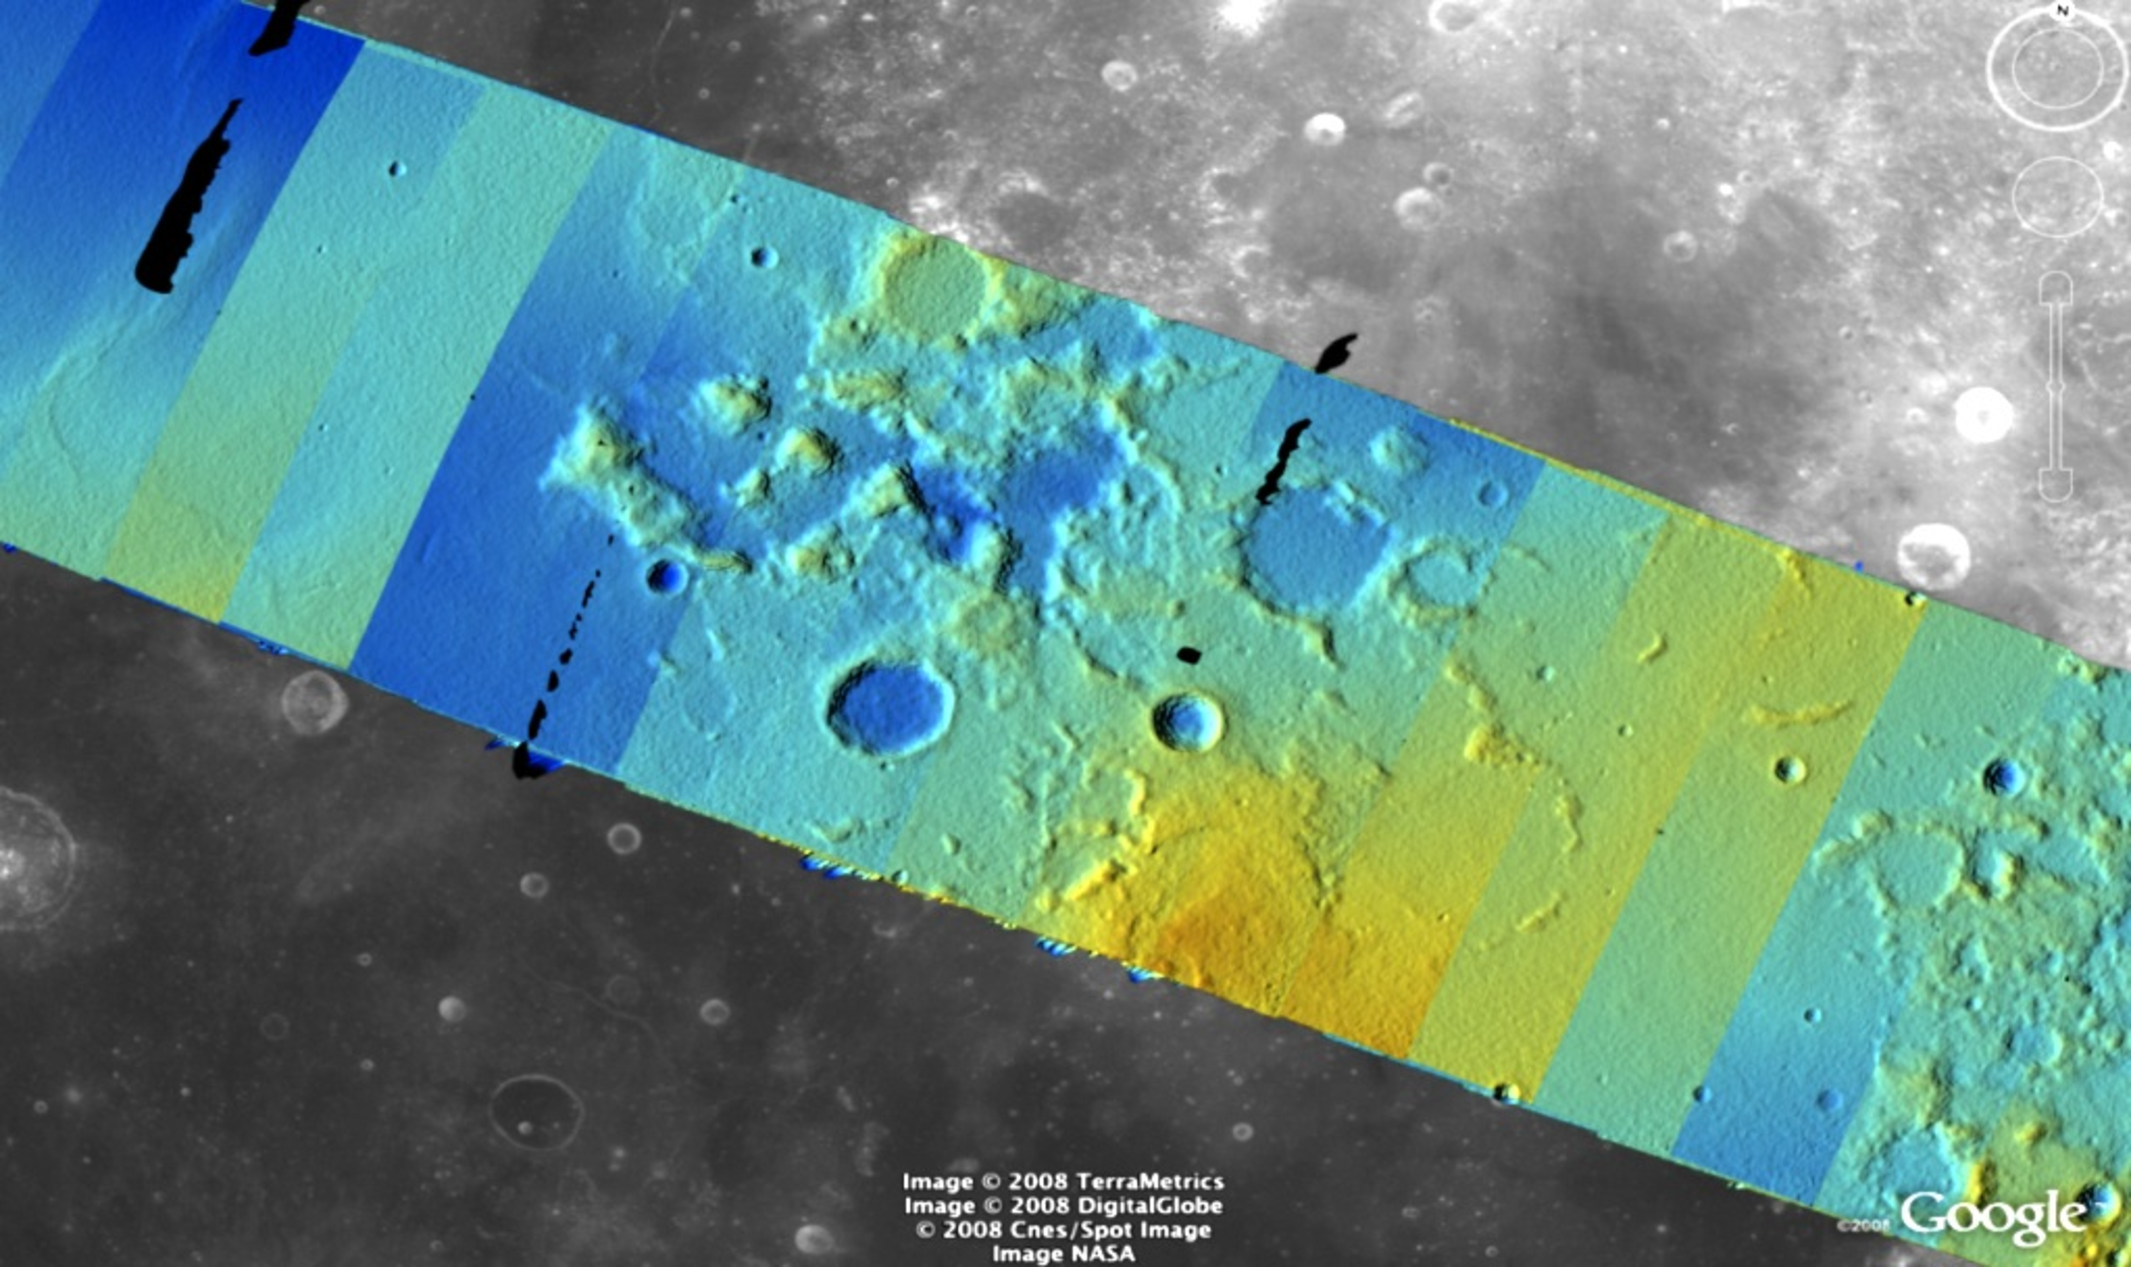
\includegraphics[width=8cm]{images/ba_orig}
  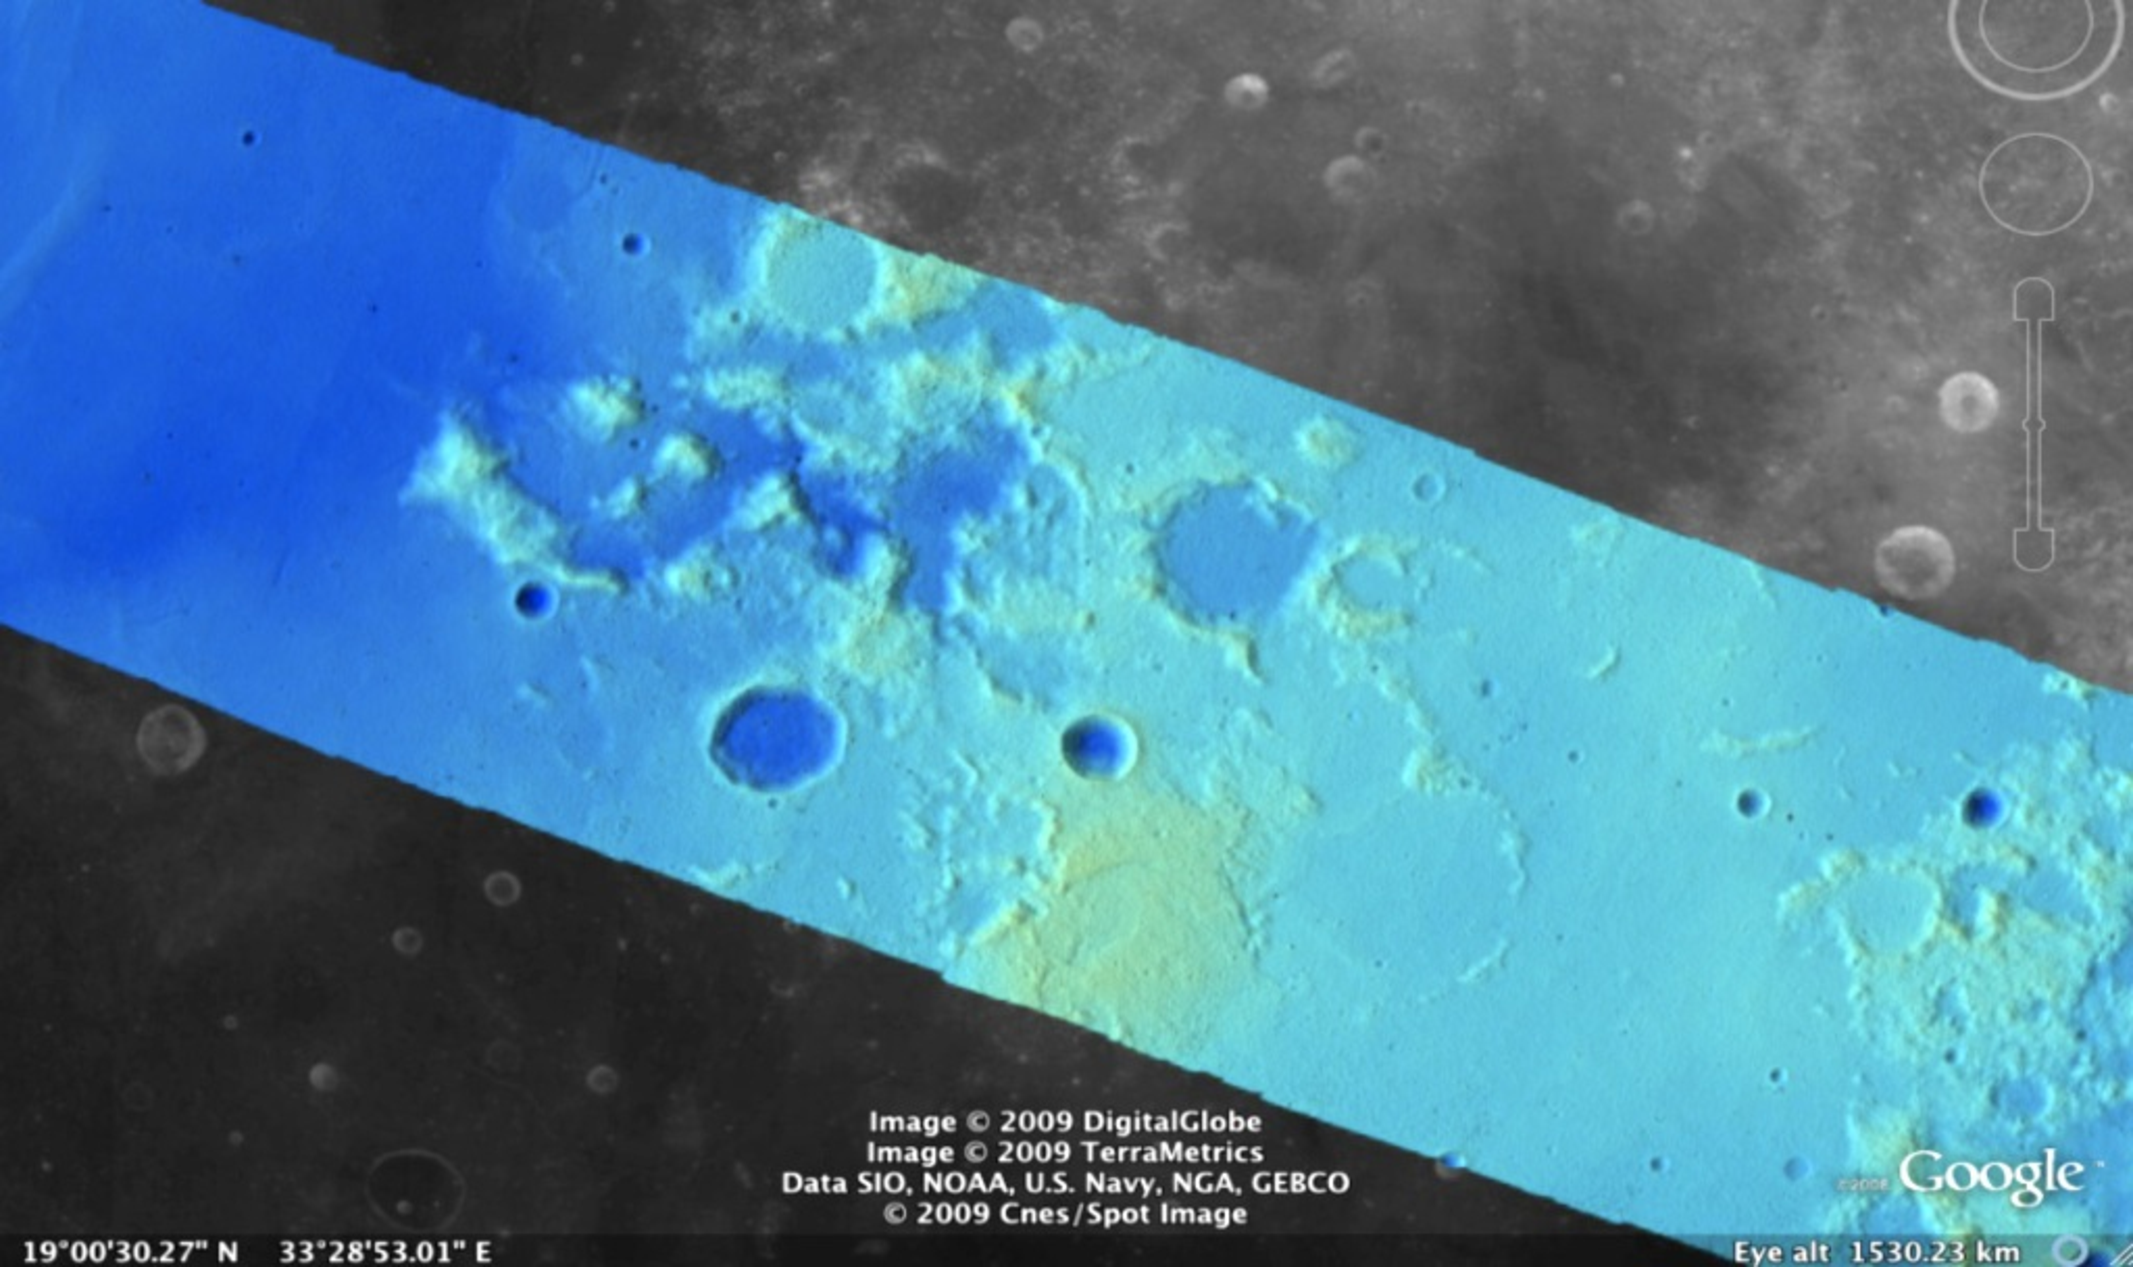
\includegraphics[width=8cm]{images/ba_adjusted}
  \caption{Bundle adjustment is illustrated here using a color-mapped,
    hill-shaded DEM mosaic from Apollo 15 Orbit 33 imagery. (a)
    Prior to bundle adjustment, large discontinuities can exist between
    overlapping DEMs made from different images. (b) After bundle
    adjustment, DEM alignment errors are minimized, and no longer visible.}
  \label{fig:bundle_adjustment}
\end{figure}

Bundle adjustment can also take advantage of \acp{GCP}, which are
3D locations of features that are known a priori (often by measuring
them by hand in another existing \ac{DEM}). \acp{GCP} can improve the internal
consistency of your \ac{DEM} or align your \ac{DEM} to an existing data
product. Finally, even though bundle adjustment calculates the
locations of the 3D objects it views, only the final properties of
the cameras are recorded for use by the Ames Stereo Pipeline. Those
properties can be loaded into the \texttt{stereo} program which
uses its own method for triangulating 3D feature locations.

When using the Stereo Pipeline, bundle adjustment is an optional step
between the capture of images and the creation of \acp{DEM}. The bundle
adjustment process described below should be completed prior to
running the \texttt{stereo} command.

Although bundle adjustment is not a required step for generating
\acp{DEM}, it is {\em highly recommended} for users who plan to
create \acp{DEM} for scientific analysis and publication.  Incorporating
bundle adjustment into the stereo work flow not only results in
\acp{DEM} that are more internally consistent, it is also the correct
way to co-register your \acp{DEM} with other existing data sets and
geodetic control networks.

At the moment however, Bundle Adjustment does not automatically work
against outside DEMs from sources such as laser altimeters. Hand
picked \acp{GCP} are the only way for \acp{ASP} to register to those
types of sources.

\subsection{A deeper understanding}

In bundle adjustment the position and orientation of each camera
station are determined jointly with the 3D position of a set of image
tie-points points chosen in the overlapping regions between images.
Tie-points are automatically extracted using Vision Workbench's
Interest Point module, or alternatively the SURF robust feature
extraction algorithm \citep{surf08}. Outliers are then rejected using the
RANSAC method \citep{fischler81} and trimmed to 1000 matches that are
spread evenly across the images.

\begin{figure}[b!]
  \begin{center}
  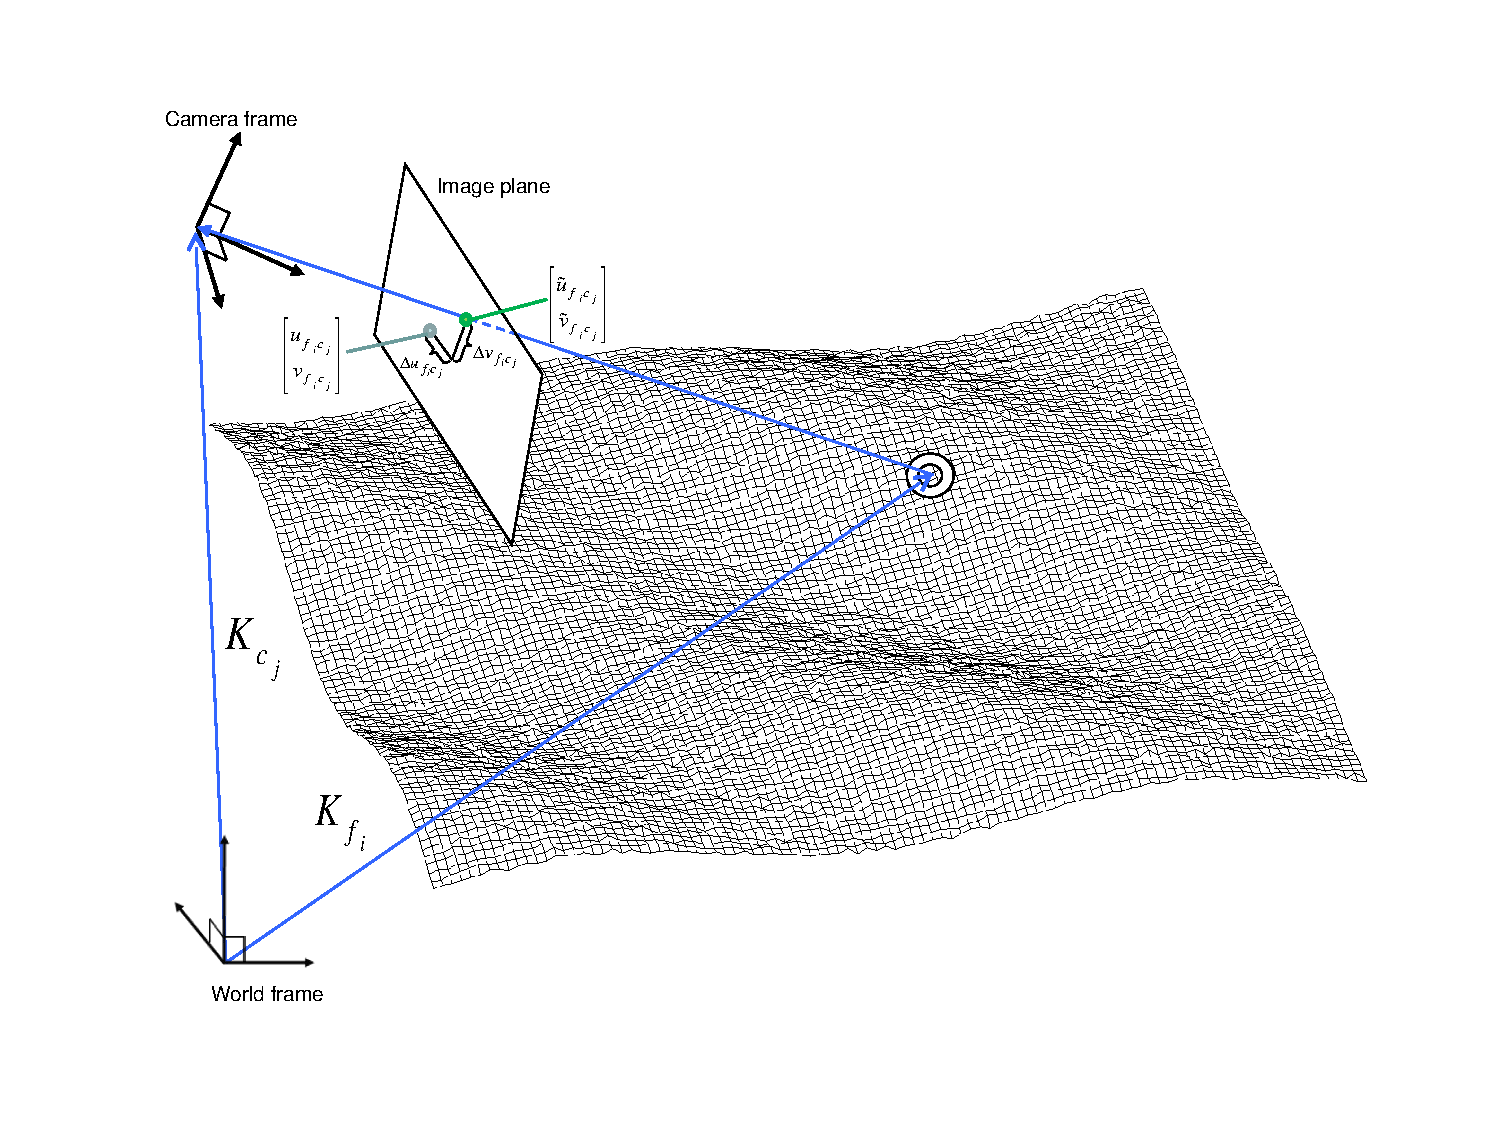
\includegraphics[trim=20mm 20mm 20mm 15mm,clip,width=6in]{images/ba_feature_observation.pdf}
  \end{center}
  \caption{ A feature observation in bundle adjustment, from \citet{moore09} }
  \label{fig:ba_feature}
\end{figure}

Our bundle adjustment approach follows the method described
in~\cite{triggs00} and determines the best camera
parameters that minimize the projection error given by ${\bf \epsilon}
= \sum_k\sum_j(I_k-I(C_j, X_k))^2$ where $I_k$ are feature locations
on the image plane, $C_j$ are the camera parameters, and $X_k$ are the
3D positions associated with features $I_k$. $I(C_j, X_k)$ is an image
formation model (i.e. forward projection) for a given camera and 3D
point. The optimization of the cost function uses the
Levenberg-Marquardt algorithm (LMA). Speed is improved by using sparse
methods as described in \citet{hartley04}.

To eliminate the gauge freedom inherent in this problem, we add two
additional error metrics to this cost function to constrain the position
and scale of the overall solution. First, ${\bf \epsilon} =
\sum_j(C_j^{initial}-C_j)^2$ constrains camera parameters to stay
relatively close to their initial values.  Second, a small handful of
3D ground control points are chosen by hand and added to the
error metric as ${\bf \epsilon} = \sum_k(X_k^{gcp}-X_k)^2$ to
constrain these points to known locations in the planetary coordinate
frame.  In the cost functions discussed above, errors are weighted by
the inverse covariance of the measurement that gave rise to the
constraint.

Like other iterative optimization methods, there are several
conditions that will cause bundle adjustment to terminate.  When
updates to parameters become insignificantly small or when the error,
${\bf \epsilon}$, becomes insignificantly small, then the algorithm
has converged and the result is most likely as good as it will get.
However, the algorithm will also terminate when the number of
iterations becomes too large, in which case bundle adjustment may or
may not have finished refining the parameters of the cameras.

\section{Performing bundle adjustment with isis\_adjust}

The \texttt{isis\_adjust} program is designed to perform bundle
adjustment on images supported by USGS's \ac{ISIS} 3 software
package.  The \texttt{isis\_adjust} program does not discriminate
based on camera type.  It can perform bundle adjustment on images
from line-scan imagers like \ac{MOC}, \ac{LROC} NAC, \ac{HiRISE},
and the \ac{CTX}.  The \texttt{isis\_adjust} program can also perform
bundle adjustment on traditional frame cameras (e.g. Apollo Metric
Camera). Theoretically it should also work with push-frame
imagers like the \ac{THEMIS} VIS, and \ac{LROC} WAC, though this is
untested.

The \texttt{isis\_adjust} program works by first converting all
pixel measurements in an image to measurements defined on the ideal
focal plane using millimeters and the \ac{ET}. The \ac{ET} is the
absolute second at which that pixel measurement was recorded on the
camera.  For a frame camera, all of the pixels are captured at the
same time so the \ac{ET} will be identical for all measurements on
the image.  For pushbroom, pushframe, or other cameras which build
up their `image' over time, different parts of the image will have
different ET values.  For example, on a MOC image between the first
and last line about 5 seconds of \ac{ET} will have elapsed.

When \texttt{isis\_adjust} calculates the partial derivatives of the
forward projection of a point, it uses an ideal pinhole camera model.
The properties of this model are defined as properties of the subject
camera at the specified \ac{ET} for the current measure plus the
correction function, $f(t)$, that \texttt{isis\_adjust} is solving
for.  Many forms of $f(t)$ could be used; the only limit is the
number of parameters in the equations. Some initial work hints that
anything greater than a second order polynomial becomes an ill-posed
problem, but we hope to investigate this further in the future.

\subsection{Options}

The following is a listing and explanation of the options that can be
given to \texttt{isis\_adjust} on the command line. These options are
not required.

\begin{description}

\item[\texttt{-\/-cnet|-c \textit{control-network-file}}] \hfill \\
  \emph{Optional.} This option will force {\tt isis\_adjust} to
  use a pre-built built control network. This control network can
  either be in the \ac{USGS} \ac{ISIS} ``cnet'' format or in the binary Vision
  Workbench format.

  If no control network is supplied using this option, {\tt
    isis\_adjust} will look for match files in the current working
  directory with base filenames that match the input images.  The
  \texttt{isis\_adjust} program will then create its own control
  network file and save it as \texttt{isis\_adjust.cnet}.

\item[\texttt{-\/-cost-function L1|L2|Cauchy|Huber|PseudoHuber(=L2)} ] \hfill \\
  Sets the cost function used for bundle adjustment. Default is \texttt{L2}
  which is the normal squared error. The full list of available options
  are:

  \begin{description}
    \item[L1] Proportional Error
    \item[L2] Squared Error and Default Option.
    \item[Cauchy]
    \item[Huber]
    \item[PseudoHuber]
  \end{description}

  The options towards the end of the list are robust cost functions
  that deal better with non-ideal data that has outliers. These robust
  cost functions are performed by post-weighting the original errors yet
  still using equations derived for squared error.

\item[\texttt{-\/-bundle-adjuster Ref|Sparse|RobustRef|RobustSparse|RobustSparseKGCP(=Sparse)}] \hfill \\
  Sets the bundle adjustment code to be used. The standard to use is
  \texttt{Sparse}, which is a traditional squared error derived method that
  utilizes sparse matrices to obtain speed. Here are the complete list
  of options:

  \begin{description}
    \item[Ref] Reference implementation that doesn't use sparse methods.
    \item[Sparse] Default implementation.
    \item[RobustRef]
    \item[RobustSparse]
    \item[RobustSparseKGCP]
  \end{description}

  The ending methods are experimental student-t derived bundle
  adjustment algorithms. Using the experimental robust algorithm
  overrides the {\tt cost-function} option. The last two bundle
  adjustment algorithms are still experimental and are a work in
  progress.

\item[\texttt{-\/-disable-camera-const}] \hfill \\
  \emph{Optional.} This disables the camera constraint error. Useful
  for debugging and just exploring what are the effects of this cost
  function.

\item[\texttt{-\/-disable-gcp-const}] \hfill \\
  \emph{Optional.} This disables the \ac{GCP} constraint error even
  if \acp{GCP} are provided. Useful for debugging and just exploring
  what the effects are of \acp{GCP}.

\item[\texttt{-\/-gcp-scalar \textit{multiplier(=1)}}] \hfill \\
  \emph{Optional.} Sets the multiplier that is used to adjust the
  sigma (or uncertainty) of the \aclp{GCP}. The sigmas of
  \aclp{GCP} are defined in the \ac{GCP} data file, so this
  option is useful when debugging for universally scaling \ac{GCP} sigmas
  up or down.

\item[\texttt{-\/-lambda|-l \textit{float}}] \hfill \\
  \emph{Optional.} This sets the starting value for $\lambda$: the
  parameter in the Levenberg Marquardt (LMA) optimization algorithm
  that selects between Gauss-Newton optimization and gradient
  descent. This parameter evolves over time on its own, but this
  argument can be used to override its initial value. \emph{This is an
  advanced setting, not recommended for normal use.}

\item[\texttt{-\/-min-matches \textit{integer(=5)}}] \hfill \\
  Set the minimum number of tie-points that are required between a
  pair of images for them to be included in the control network. This
  option is useful for eliminating tie-points from image pairs that
  have only a handful of poor or erroneous matches.

\item[\texttt{-\/-max-iterations \textit{integer(=25)}}] \hfill \\
  Sets the maximum number of iterations for bundle adjustment. The
  number of required iterations will vary by problem size, so this
  parameter allows the user to decide how much time they're willing
  to dedicate to the correction of the data.  We have found that 20
  iterations suffices for small problems with 10 or fewer images, and
  tens or hundreds of iterations may be required for problems with
  hundreds or thousands of images.

\item[\texttt{-\/-poly-order \textit{integer(=0)}}] \hfill \\
  \emph{Optional.} Sets the order of the polynomial that is used for
  adjustment. Using zero means only apply offset to the camera
  parameters that are not time dependent. That setting is recommend
  for frame cameras. Linescan imagers should using either a first
  order polynomial or a second order. Increasing this number too high can
  lead to a problem that is ill-defined and would prevent the algorithm 
	from converging on a solution. \emph{Initial work suggest that anything
    beyond a 2nd order polynomial would be ill-defined. 3rd order may
    work with a good dose of ground control points.}

\item[\texttt{-\/-position-sigma \textit{float(=100)}}] \hfill \\
  Sets the sigma (or uncertainty) of the spacecraft position in
  units of meters.

\item[\texttt{-\/-pose-sigma \textit{float(=0.1)}}] \hfill \\
  Sets the sigma (or uncertainty) of the spacecraft pose in units
  of radians.

\item[\texttt{-\/-report-level|-r \textit{integer(=10)}}] \hfill \\
  \emph{Optional.} Sets the report level for the final bundle
  adjustment report.  This report is saved as
  \texttt{isis\_adjust.report}. Report levels available are:

  \begin{description}
    \item[0   - CommandLine Error and Final report]
    \item[10  - CommandLine Iteration Error (default)]
    \item[20  - Write Report file]
    \item[25  - \textnormal{\emph{In development}}]
    \item[30  - Write Stereo Triangulation Error]
    \item[35  - \textnormal{\emph{In development}}]
    \item[100 - Debug, Write Error Vectors (big human readable)]
    \item[110 - Debug, Write Jacobian Matrix (massive human readable)]
  \end{description}

\item[\texttt{-\/-robust-threshold \textit{float(=10)}}] \hfill \\
  Sets the robust threshold; an additional parameter specifically for
  the \texttt{PseudoHuber}, \texttt{Huber}, and \texttt{Cauchy} arguments to the   \texttt{-\/-cost-function} option.

\item[\texttt{-\/-save-iteration-data|-s}] \hfill \\
  \emph{Optional.} Use to write {\tt bundlevis} visualization files.

\item[\texttt{-\/-seed-with-previous}] \hfill \\
  \emph{Optional.} Loads up the previous {\tt isis\_adjust} session's
  adjustment file and uses them as a starting point for this session.

\item[\texttt{-\/-write-isis-cnet-also}] \hfill \\
  \emph{Optional.} Write an \ac{ISIS} \ac{PVL} style control network file to
  \texttt{isis\_adjust.net}. The output file is very large compared to
  the binary output, \texttt{isis\_adjust.cnet}, but is human readable
  and compatible with the \ac{ISIS} 3 \texttt{qnet} tool.

\item[\texttt{-\/-write-kml [0|1(=0)]}] \hfill \\
  \emph{Optional.} Providing this option with a zero will have the
  program write a \ac{KML} file showing the location of all the \acp{GCP}
  and be colored according to their final error. Providing this
  option with a one will have this perform as before, but also have it
  write all of the 3D point estimates. This is useful for debugging and
  for having a quick visualization of where stress points might exist in
  a bundle adjustment problem when there are many cameras.

\item[\texttt{-\/-help|-h}] \hfill \\
  Provides a shortened list of the above.

\end{description}

\section{Visualizing bundle adjustment with bundlevis}

The \texttt{bundlevis} program is used to visualize the process of
bundle adjustment. It will show an animated, fully interactive 3D
scene containing all the 3D points and cameras across all iterations
of bundle adjustment.  This tool is used to quickly determine if
bundle adjustment was successful.  If something does go wrong,
\texttt{bundlevis} can be a powerful debugging tool for identifying
the problem.

\begin{figure}[b!]
  \begin{center}
  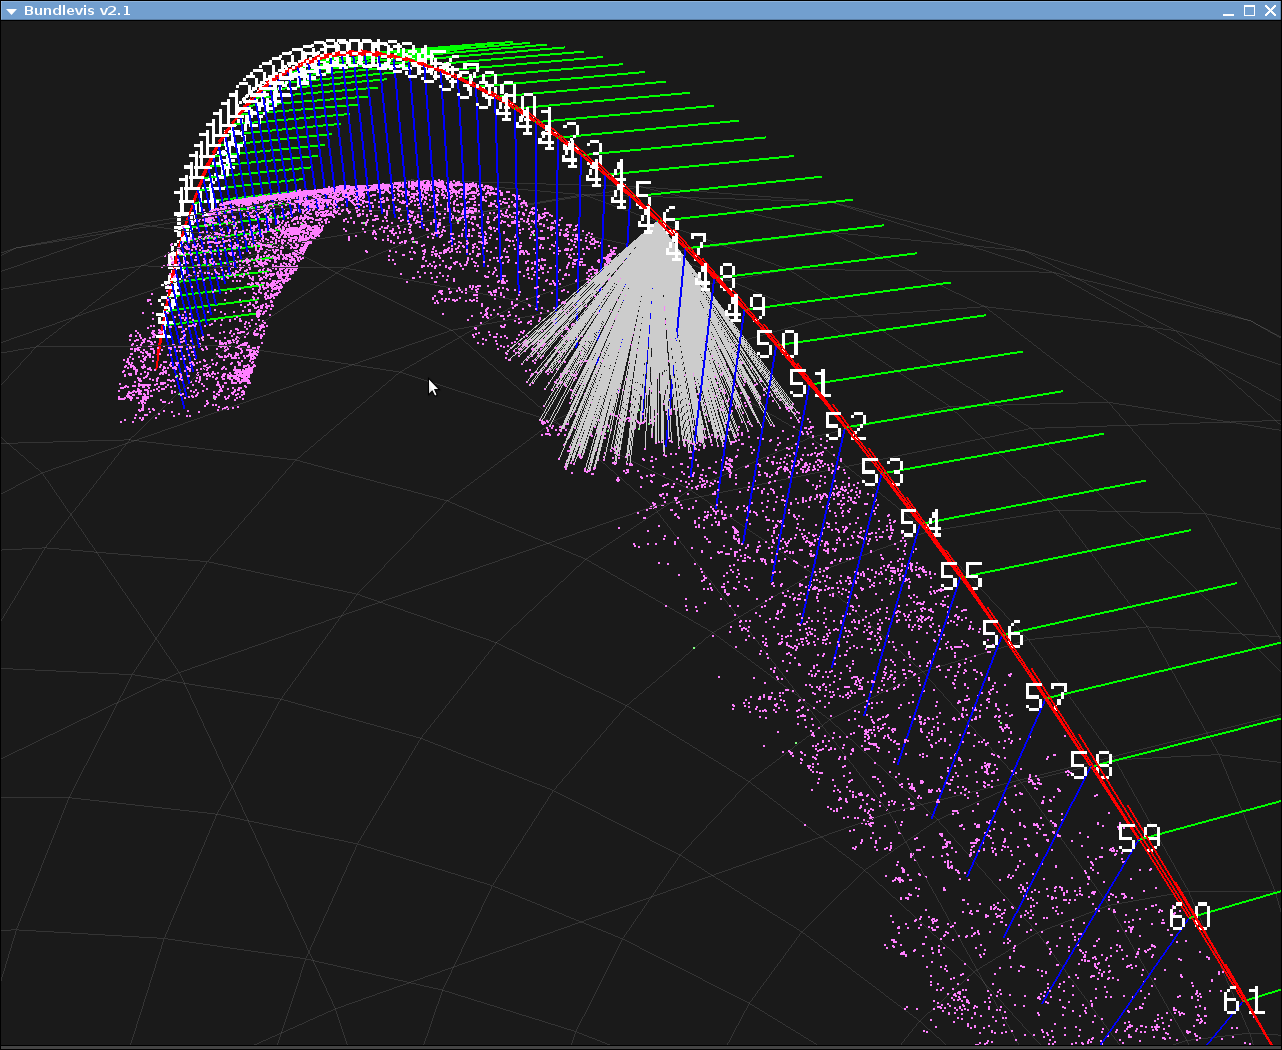
\includegraphics[width=5in]{images/bundlevis_apollo.png}
  \end{center}
  \caption{ A screenshot of \texttt{bundlevis} visualizing the bundle
    adjustment of imagery from the Apollo 15 Metric Camera (orbit
    33). }
  \label{fig:bundlevis}
\end{figure}

Once \texttt{bundlevis} has loaded the data from a bundle adjustment run,
the user can click on and inspect the position of 3D points that are
in purple and play back the iterations using the keyboard. Double
clicking on a camera will cause lines to be drawn to each point viewed
by the camera. Clicking on a 3D point causes lines to be drawn to all
cameras that view the point.

Bundle adjustment can fail in a variety of different ways, but users
should be aware of two common failure modes.  The first is segmentation;
where tie points will split into two or more distinct groups,
producing cliffs between or clumps among points. This is usually
caused by insufficient matches between a pair of images in your
control network.  You may need to choose some tie-points between
these images by hand or add additional images that overlap with the
problem area.

The second common sign of a failure is a point cloud explosion or
implosion (the resulting terrain looks unrecognizably noisy). This
most often results from a high number of outlying, bad tie-point
measurements. These bad constraints can be removed by hand or
mitigated using one of the robust cost modes (e.g. by using the
\texttt{-\/-cost-function} argument for \texttt{isis\_adjust}).

\subsection{Options}

The following is a listing and explanation of the options
that can be given to \texttt{bundlevis} from the command line.

\begin{description}

\item[\texttt{-\/-camera-iteration-file|-c \textit{bundlevis-camera-iteration-file}}] \hfill \\
  \emph{Optional.} Supply a camera iteration file that was produced by
       \texttt{isis\_adjust}.  \texttt{bundlevis} will only draw cameras
       if you supply a camera iteration file.

\item[\texttt{-\/-points-iteration-file|-p \textit{bundlevis-point-iteration-file}}] \hfill \\
  \emph{Optional.} Supply a point iteration file that was produced by
       \texttt{isis\_adjust}.  \texttt{bundlevis} will only draw 3D points
       if you supply a point iteration file.

\item[\texttt{-\/-control-network-file|-n \textit{Vision-Workbench-binary-control-network-file}}] \hfill \\
  \emph{Optional.} Supply a control network file that was produced by
       {\tt isis\_adjust}.  This allows {\tt bundlevis} to show the
       relationship between points and cameras when used in
       conjunction with \texttt{-\/-camera-iteration-file} and
       \texttt{-\/-points-iteration-file}.

\item[\texttt{-\/-additional-pnt-files \textit{bundlevis-point-iteration-files}}] \hfill \\
  \emph{Optional.} Supply additional points to be animated alongside
  the camera and 3D points.  The files given must be in the same
  format as a \texttt{bundlevis} point iteration file and have the same number
  of iterations.

\item[\texttt{-\/-fullscreen}] \hfill \\
  \emph{Optional.} Displays \texttt{bundlevis} using the entire screen;
  otherwise the program loads in a window. \emph{The fullscreen option
    does not work correctly with dual screen systems.}

\item[\texttt{-\/-stereo}] \hfill \\
  \emph{Optional.} Render the 3D scene in red/blue anaglyph mode.

\item[\texttt{-\/-show-moon}] \hfill \\
  \emph{Optional.} Draws a wireframe sphere with a radius of 1737.3~km
  that represents the Moon.

\item[\texttt{-\/-show-mars}] \hfill \\
  \emph{Optional.} Draws a wireframe sphere with a radius of 3397~km
  that represents Mars.

\item[\texttt{-\/-show-earth}] \hfill \\
  \emph{Optional.} Draws a wireframe sphere that represents the Earth.

\end{description}

\subsection{Controls}

Once \texttt{bundlevis} is running, there are several controls that
can be used to interface with the program. There are the playback
controls, jump-to-frame controls, and the mouse.

\paragraph{Playback Controls}

Playback controls are similar to those in the popular Winamp program;
arranged on the keyboard like the controls on a tape deck.

\newenvironment{myindentpar}[1]
               {\begin{list}{}
                   {\setlength{\leftmargin}{#1}}
                 \item[]
               }
               {\end{list}}

\begin{myindentpar}{3cm}
\begin{description}
  \item[Z] Step back one iteration
  \item[X] Play
  \item[C] Pause
  \item[V] Stop \emph{(which is the same as Pause except that
    bundlevis goes back to iteration 0)}
  \item[B] Step forward one iteration
\end{description}
\end{myindentpar}

\paragraph{Jump-to-Frame Controls}
Jump-to-Frame controls are the numbers \textbf{1-9} along the top of
the keyboard. Pressing \textbf{1} will display the very first
iteration. Pressing \textbf{9} will display the very last
iteration. Pressing \textbf{2} through \textbf{8} will display
iterations that are somewhere in between based on the value of the
number. Finally, pressing \textbf{0} will cause \texttt{bundlevis} to
display the points at their very last iteration with an additional
tail pointing back to the starting position of the points in the first
iteration.

\paragraph{Mouse}
The mouse is used to move around the model, and has the same controls
found in many 3D environments (e.g. \texttt{osgviewer}). Moving the
mouse with the \textbf{left mouse button} held down will cause the
model to rotate.  Moving with the \textbf{right mouse button} pressed
will zoom, and moving with the \textbf{middle mouse button} will
translate. Alternatively for systems where the mouse is
button-challenged, \textbf{option + mouse} is translation and
\textbf{command + mouse} is zoom.

Double clicking with the mouse on a point or camera will allow the
user to query entities in the model.  A double click will cause the
point number and camera number to be printed to the terminal. The
number identifier for a given camera or point will also appear when
the viewer is zoomed in on that entity.

\section{Examples of Use}
\label{sec:ba_example}

\subsection{Processing Mars Orbital Camera}

What follows is an example of bundle adjustment using two \ac{MOC}
images of the south Cydonia region. We use images M10/00254 and
R09/01059. These images are available from NASA's \ac{PDS} (the
\ac{ISIS} \texttt{mocproc} program will operate on either the IMQ
or IMG format files, we use the \texttt{.imq} below in the example).
For reference, the following \ac{ISIS} commands are how to convert
the \ac{MOC} images to \ac{ISIS} cubes.

\begin{verbatim}
  ISIS 3> mocproc from= m1000254.imq to= m1000254.cub mapping=no
  ISIS 3> mocproc from= r0901059.imq to= r0901059.cub mapping=no
\end{verbatim}

You will note that the resulting images are not map projected. Bundle
adjustment requires the ability to project arbitrary 3D points into
the camera frame. The process of map projecting an image dissociates
the camera model from the image. Map projecting can be perceived as
the generation of a new infinitely large camera sensor that is
perfectly parallel to the surface of its subject ( and thus spherical
). At this point it's extremely hard to project a random point into
the camera's image. The math would follow the transformation from
projection into the camera frame, then projected back down to surface
that ISIS uses, then finally up into the infinitely large sensor. The
\texttt{isis\_adjust} program does not support this.

At this point in order, we need to automatically generate tie-points between
these two images.  This can be done using the \texttt{ipfind} and
\texttt{ipmatch} utilities.  These tools do not (currently) work
with photometrically calibrated images, so we must first convert
these images to a standard format using the \ac{ISIS} program
\texttt{isis2std}:

\begin{verbatim}
  ISIS 3> isis2std from= m1000254.cub to= m1000254.png format= PNG
  ISIS 3> isis2std from= r0901059.cub to= r0901059.png format= PNG
\end{verbatim}

Here is how to process those newly created PNG files for tie-points
using the Interest Point Module tools from Vision Workbench.

\begin{verbatim}
  > ipfind  m1000254.png r0901059.png --int obalog --des sgrad -g 1.2
  > ipmatch m1000254.png r0901059.png -d -r homography -i 30
\end{verbatim}

\begin{center}
\fcolorbox{black}{lgray}{ \begin{minipage}{5.5in}

    We are aware that the tie-point tools available in Vision
    Workbench do not always produce enough matches for bundle
    adjustment. An alternative that we have found that works quite
    well is to use an outside method such as SURF \citep{surf08}. We
    have included a small example program that converts SURF output to
    a Vision Workbench style match file.  \\ \\ For this example it is
    okay to use the results from \texttt{ipfind} and
    \texttt{ipmatch}. Expect to find approximately 100 matched
    points. Your results will be slightly different due to the random
    nature of RANSAC.

\end{minipage}}
\end{center}

Finally it is time to start bundle adjustment. There are many options
that can be used at this stage.  We have chosen those required to
create visualization data for \texttt{bundlevis}.  We have also set
the maximum iterations to 100 and chosen the option to create a
detailed report file of \texttt{isis\_adjust}'s results.

\begin{verbatim}
  ISIS 3> isis_adjust *.cub -s --max 30 -r 50
\end{verbatim}

This command will produce considerable debugging output and will
place many output files in the current working directory. Don't
panic--this is perfectly normal! If you look through the output in
the terminal or alternatively in the output report file,
\texttt{isis\_adjust.report}, you'll see that the problem did not
converge but reduced most of the error in the first 40 iterations
(again, your results may vary slightly). The lack of convergence
is worrisome and a few (like 3) ground control points would probably
help considerably.  Notice that the error improved only slightly
after those first 40 iterations, but the shape of the pointcloud and
the camera paths changed considerably. This untwisting of the
cameras can be seen next in \texttt{bundlevis}.

Visualizing all of the data that was exported for \texttt{bundlevis}
can be carried out as follows:

\begin{verbatim}
  > bundlevis -p iterPointsParam.txt -c iterCameraParam.txt \
              -n isis_adjust.cnet
\end{verbatim}

Press escape to exit out of \texttt{bundlevis} when finished.  You may
also want to try viewing the data with a wireframe of Mars to give
some perspective. Note, you will have to zoom in very far since the
size of a MOC frame is quite small relative to the size of Mars!

\begin{verbatim}
  > bundlevis -p iterPointsParam.txt -c iterCameraParam.txt \
              -n isis_adjust.cnet --show-mars
\end{verbatim}

Producing a DEM using the newly created corrections is the same as
covered in the Tutorial on page \pageref{ch:tutorial}, with one small
difference: \texttt{stereo} needs to know of the existence of the
correction files, \texttt{m1000254.isis\_adjust} and
\texttt{r0901059.isis\_adjust}.  The \ac{MOC} images should also be 
map-projected with \texttt{cam2map} (as the Tutorial shows) to create
the \texttt{.map.cub} files that \texttt{stereo} will operate on.

\begin{verbatim}
  ISIS 3> stereo m1000254.map.cub r0901059.map.cub m1000254.isis_adjust \
                 r0901059.isis_adjust MOC_RESULTS/M1000254_R0901059
\end{verbatim}

Note the two new arguments (\texttt{*.isis\_adjust}) to
\texttt{stereo} that provide it with the necessary corrections. When
providing outside camera models for images, they are always the 3rd
and 4th argument for \texttt{stereo}.

\subsection{Processing with Ground Control Points}

Ground control point files describe a single point in the world
that is seen by 1 or more cameras. How they are measured in the
first place is up to the user. We use a manual process of comparing
each image to a respected map projected image and then recording
the latitude, longitude, and altitude of the point(s). The maps to
register against can be anything, but it is recommended to register
against a product with a high amount of cartographic stability and
accuracy.  For terrestrial work, we would use a \ac{USGS} product
that can provide imagery that is registered to LIDAR height
measurements.

Unlike match files, ground control points must specifically be given
to \texttt{isis\_adjust} from the command line, but in no particular
order. Ground control point files are written with the extension
\texttt{.gcp}. Below is an example of a ground control point file that
was created to control a series of Apollo Metric Camera images from
several Apollo 15 orbits.

\begin{verbatim}
    -52.8452 27.2561 1735999 300 300 500
    sub4-AS15-M-2086.cub     210.9   3565.0
    sub4-AS15-M-2087.cub     1476.9  3579.0
    sub4-AS15-M-2088.cub     2798.9  3586.8
    sub4-AS15-M-2089.cub     4133.5  3588.6
    sub4-AS15-M-2344.cub     906.9   3874.8
    sub4-AS15-M-2345.cub     2204.2  3913.9
    sub4-AS15-M-2482.cub     939.8   4348.0
    sub4-AS15-M-2483.cub     2282.0  4340.7
    sub4-AS15-M-2484.cub     3642.1  4330.9
\end{verbatim}

The first line of a \texttt{.gcp} file is like a header line and
is different from the remaining lines.  The first line defines the
world location of the ground control point, and the rest of the
lines define the image locations of the ground control points. Here
are what the columns mean for the first line.

\begin{myindentpar}{2cm}
\begin{description}
  \item[Column 1:] Longitude in degrees
  \item[Column 2:] Latitude in degrees
  \item[Column 3:] Radius in meters
  \item[Column 4:] Sigma (or uncertainty) in meters for Local X axis
  \item[Column 5:] Sigma (or uncertainty) in meters for Local Y axis
  \item[Column 6:] Sigma (or uncertainty) in meters for Local Z axis
\end{description}
\end{myindentpar}

The other lines describe where this \ac{GCP} is found in each image:

\begin{myindentpar}{2cm}
\begin{description}
  \item[Column 1:] Image name
  \item[Column 2:] Sample (X) image measurement
  \item[Column 3:] Line (Y) image measurement
\end{description}
\end{myindentpar}

Make a {\tt .gcp} file for every ground control point, then be sure
to feed them as an input to {\tt isis\_adjust}. Remember that you
can scale the sigma of all ground control points by using the {\tt
-\/-gcp-scalar} flag. This can save time by allowing you to make
adjustments without needing to edit all of the files individually.

\subsection{Sharing Data with ISIS 3's qnet program}

\ac{ISIS} contains a program called \texttt{qnet} whose purpose is
to create and edit \ac{ISIS} style control network files. To share
a control network with \texttt{qnet}, you will need to save our
control network in the \ac{ISIS} format. If bundle adjustment has
already been performed once and if we want to simply convert the
control network for use in \texttt{qnet}, you can use this command
to save an \ac{ISIS} style control network:

\begin{verbatim}
  ISIS 3> isis_adjust -c isis_adjust.cnet --write-isis-cnet-also *.cub
\end{verbatim}

Otherwise if this is the first time performing bundle adjustment and a
control network does not already exist, use:

\begin{verbatim}
  ISIS 3> isis_adjust --write-isis-cnet-also *.cub
\end{verbatim}

There should now be an \texttt{isis\_adjust.net} file in the project's
directory. It will be quite a bit larger than the other control
network file since it is stored as ASCII text, but it can be read
and edited with a text editor. Before starting \texttt{qnet}, there
is one additional preparation that must be performed. \ac{ISIS}'s
\texttt{qnet} requires a text file listing of all the cubes used
by the control network. Here's how to create one:

\begin{verbatim}
  > ls *.cub > list_of_cubes.lis
\end{verbatim}

Now, start up \texttt{qnet} without any command line arguments. Click
File$\rightarrow$Open. It will first ask for the list of cubes. Refer
it to the newly created \texttt{list\_of\_cubes.lis}. Next it will ask for
the control network. Give it \texttt{isis\_adjust.net}.

\begin{center}
\fcolorbox{black}{lgray}{ \begin{minipage}{5.5in}

    At this time \texttt{qnet} does not work with the Apollo Metric
    Camera's cube files. When loading the text file listing of cubes
    it will issue an error about invalid serial numbers for the listed
    cube files.  % (03/11/09)

\end{minipage}}
\end{center}

When finished, save the new control network file. Here's how to use
the new control network in \texttt{isis\_adjust}:

\begin{verbatim}
  ISIS 3> isis_adjust -c the_new_control_network.net *.cub
\end{verbatim}

Take note that to distinguish \ac{ISIS} style control network files
from Stereo Pipeline style control network files is by the file
extension. \ac{ISIS} control networks have the extension of
\texttt{.net} and can be read with a text editor. Stereo Pipeline's
control networks have the extension \texttt{.cnet} and are binary
format files.
